\section{Introduction -- Vijay Banerjee}
I am currently in the 2nd year of PhD program in Computer Science. My research focuses on
security in real-time cyber-physical systems (CPS). I am working on integrating detection,
prevention, and recovery strategies in CPS with real-time guarantees for security and time-
critical applications like flight software. I also like to explore real-time scheduling theory and
implementation challenges in real-time operating systems (RTOS). I genuinely smile when I work on these
ideas, unlike my photo in Fig. 1.
My goal for this course is to understand the general research methodologies used in computer
science (CS) to expand my idea of research and find my paradigm
of research. I am also looking forward to learning the best practices of research and the
common tools that are used across different disciplines to improve efficiency. Through the
class activities and interaction with my peers, I will be able to see different perspectives and
interests, which can open doors to future collaborations and intriguing discussions.
I enjoy playing classical music on the flute in my free time. I also enjoy cooking different
cuisines whenever I find an opportunity
\begin{figure}[h]
    \centering
    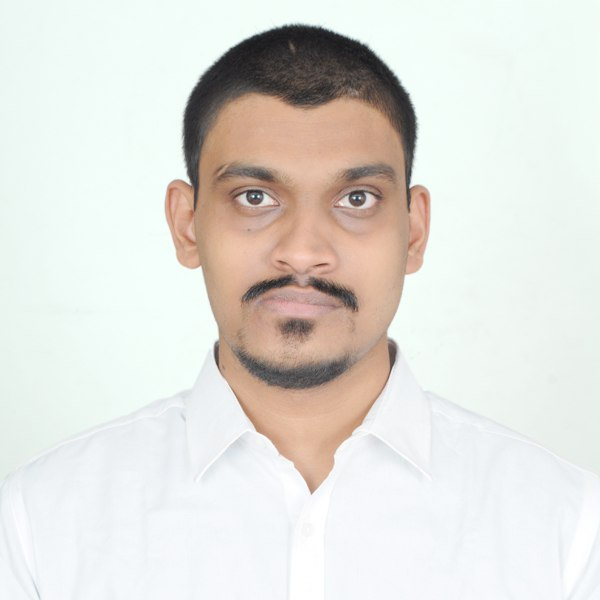
\includegraphics{banerjee.jpeg}
    \caption{This is me (I am not this grumpy in real life)}
    \label{fig:me}
\end{figure}


\section{Related Code Repo}

I am working with Real-Time Operating Systems. One of the most prominent hard RTOS is Real-Time Executive for Multiprocessor Systems (RTEMS). RTEMS has been an open-source organization for over $25$ years, and the code can be found in the following repository:
\url{https://github.com/RTEMS/rtems}



\section{Questions}
